\documentclass{standalone}
\usepackage{tikz}
\usetikzlibrary{matrix}
\usetikzlibrary{intersections, positioning, calc}
\usetikzlibrary{arrows,decorations.markings}
  
 \usetikzlibrary{arrows.meta}
 \tikzset{>={Latex[width=0.2cm,length=0.2cm, scale=2.0]}}

\tikzset{
  font={\fontsize{25pt}{12}\selectfont}}
 
\begin{document}
   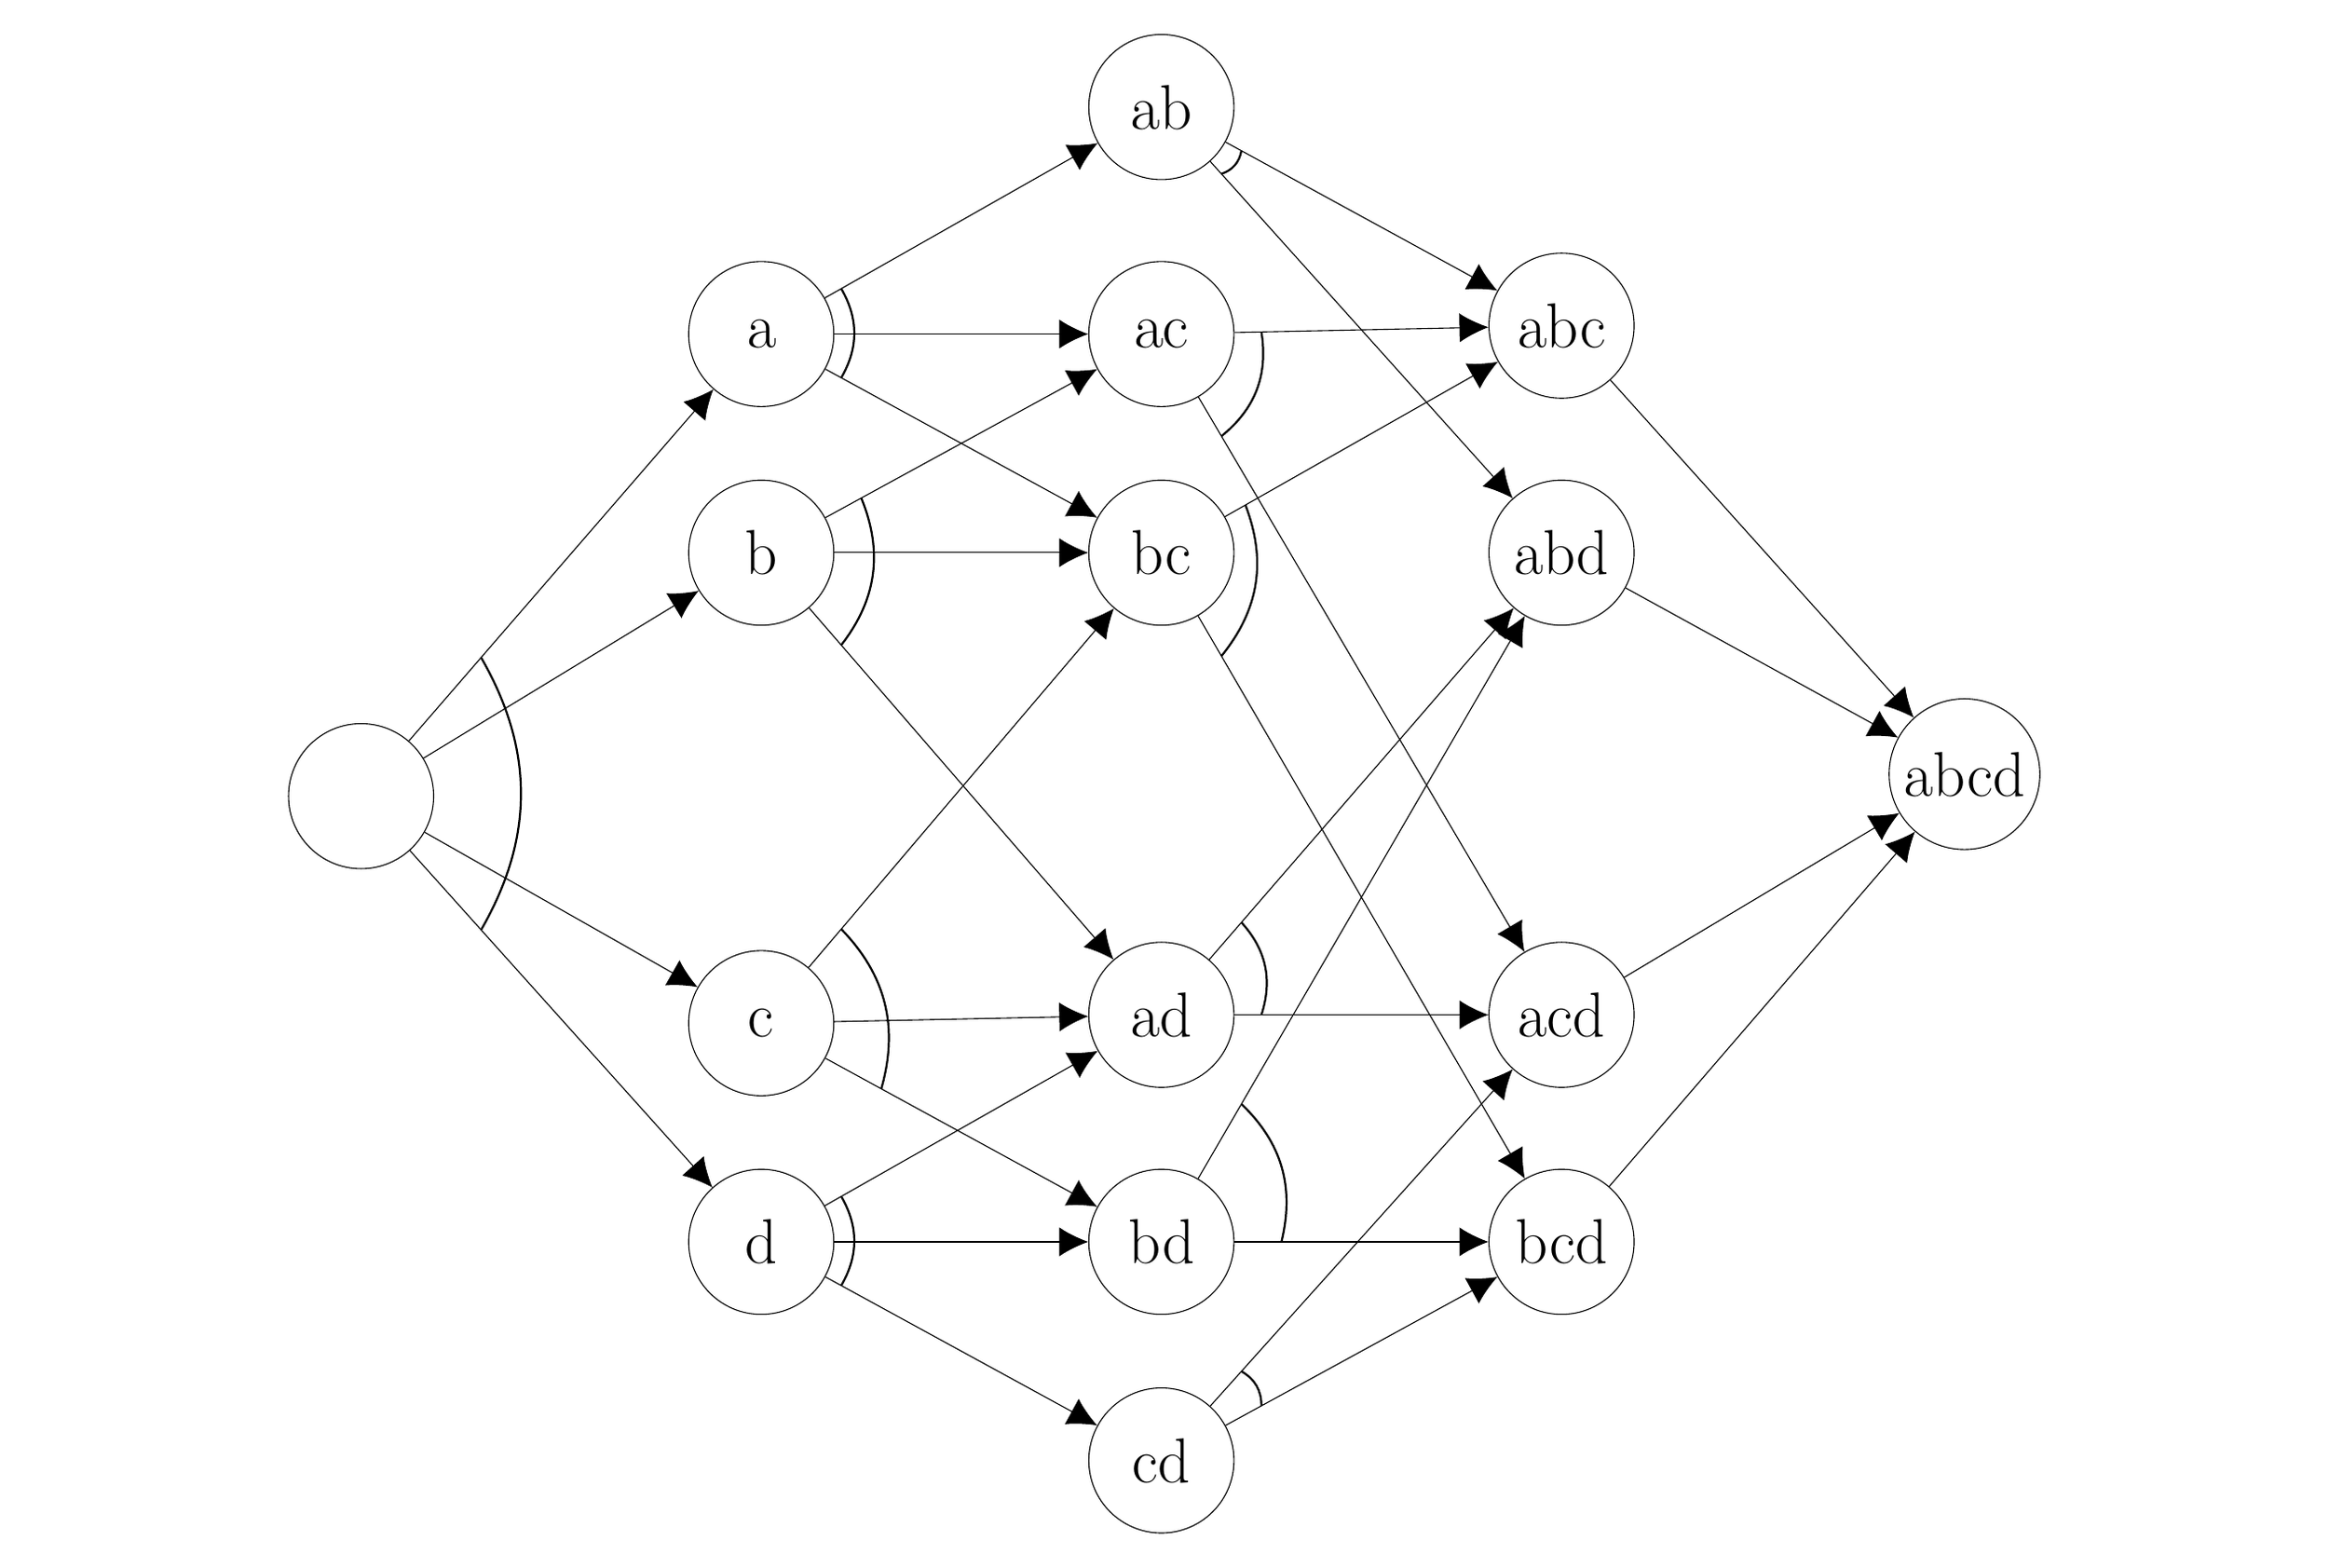
\begin{tikzpicture}[->=Latex,  sloped]
     \matrix (tree) [%
       matrix of nodes,
       minimum size=1cm,
       column sep=3.5cm,
       row sep=1cm,
       nodes = {minimum size=2cm, draw=black, shape=circle},
     ]
     {
           &     &      & ab  &     &   & \\
           &     & a   & ac  & abc &   & \\
           &     &  b  & bc  & abd &   & \\
           &  ~ &      &     &     &abcd &\\
           &     &  c  & ad  & acd &   &\\
           &     &  d  & bd  & bcd &   & \\
           &     &      &  cd  &    &   & \\
     };
     \draw[->] (tree-4-2) -- (tree-2-3);
     \draw[->] (tree-4-2) -- (tree-3-3);
     \draw[->] (tree-4-2) -- (tree-5-3);
     \draw[->] (tree-4-2) -- (tree-6-3);
     
     %%
     \draw[->] (tree-2-3) -- (tree-1-4);
     \draw[->] (tree-2-3) -- (tree-2-4);
     \draw[->] (tree-2-3) -- (tree-3-4);
     
     \draw[-, thick] ($(tree-2-3)!0.2!(tree-1-4)$) to [bend left=30] ($(tree-2-3)!0.2!(tree-3-4)$);
     
     \draw[->] (tree-3-3) -- (tree-2-4);
     \draw[->] (tree-3-3) -- (tree-3-4);
     \draw[->] (tree-3-3) -- (tree-5-4);
     \draw[-, thick] ($(tree-3-3)!0.25!(tree-2-4)$) to [bend left=30] ($(tree-3-3)!0.2!(tree-5-4)$);
     
     \draw[->] (tree-5-3) -- (tree-3-4);
     \draw[->] (tree-5-3) -- (tree-5-4);
     \draw[->] (tree-5-3) -- (tree-6-4);
     \draw[-, thick] ($(tree-5-3)!0.2!(tree-3-4)$) to [bend left=30] ($(tree-5-3)!0.3!(tree-6-4)$);
     
     \draw[->] (tree-6-3) -- (tree-5-4);
     \draw[->] (tree-6-3) -- (tree-6-4);
     \draw[->] (tree-6-3) -- (tree-7-4);
     \draw[-, thick] ($(tree-6-3)!0.2!(tree-5-4)$) to [bend left=30] ($(tree-6-3)!0.2!(tree-7-4)$);
     %%
     
     \draw[->] (tree-1-4) -- (tree-2-5);
     \draw[->] (tree-1-4) -- (tree-3-5);
     \draw[-, thick] ($(tree-1-4)!0.2!(tree-2-5)$) to [bend left=30] ($(tree-1-4)!0.15!(tree-3-5)$);
     
     \draw[->] (tree-2-4) -- (tree-2-5);
     \draw[->] (tree-2-4) -- (tree-5-5);
     \draw[-, thick] ($(tree-2-4)!0.25!(tree-2-5)$) to [bend left=30] ($(tree-2-4)!0.15!(tree-5-5)$);
     
     \draw[->] (tree-3-4) -- (tree-2-5);
     \draw[->] (tree-3-4) -- (tree-6-5);
     \draw[-, thick] ($(tree-3-4)!0.21!(tree-2-5)$) to [bend left=30] ($(tree-3-4)!0.15!(tree-6-5)$);
     
     \draw[->] (tree-5-4) -- (tree-3-5);
     \draw[->] (tree-5-4) -- (tree-5-5);
     \draw[-, thick] ($(tree-5-4)!0.2!(tree-3-5)$) to [bend left=30] ($(tree-5-4)!0.25!(tree-5-5)$);
     
     \draw[->] (tree-6-4) -- (tree-3-5);
     \draw[->] (tree-6-4) -- (tree-6-5);
     \draw[-, thick] ($(tree-6-4)!0.2!(tree-3-5)$) to [bend left=30] ($(tree-6-4)!0.3!(tree-6-5)$);
     
     \draw[->] (tree-7-4) -- (tree-5-5);
     \draw[->] (tree-7-4) -- (tree-6-5);
     \draw[-, thick] ($(tree-7-4)!0.2!(tree-5-5)$) to [bend left=30] ($(tree-7-4)!0.25!(tree-6-5)$);
     
     %%
     \draw[->] (tree-2-5) -- (tree-4-6);
     \draw[->] (tree-3-5) -- (tree-4-6);
     \draw[->] (tree-5-5) -- (tree-4-6);
     \draw[->] (tree-6-5) -- (tree-4-6);
     
     
     \draw[-, thick] ($(tree-4-2)!0.3!(tree-2-3)$) to [bend left=30] ($(tree-4-2)!0.3!(tree-6-3)$);
     

      	 %\pgfmathtruncatemacro{\xm}{\x - 1}
          %  \pgfmathtruncatemacro{\xp}{\x + 1}
          
   \end{tikzpicture}
\end{document}